\documentclass[twocolumn,a4j]{jsarticle}
\setlength{\topmargin}{-20.4cm}
\setlength{\oddsidemargin}{-10.4mm}
\setlength{\evensidemargin}{-10.4mm}
\setlength{\textwidth}{18cm}
\setlength{\textheight}{26cm}

\usepackage[top=15truemm,bottom=25truemm,left=20truemm,right=20truemm]{geometry}
\usepackage[latin1]{inputenc}
\usepackage{amsmath}
\usepackage{amsfonts}
\usepackage{amssymb}
\usepackage[dvipdfmx]{graphicx}
\usepackage[dvipdfmx]{color}
\usepackage{listings}
\usepackage{listings,jvlisting}
\usepackage{geometry}
\usepackage{framed}
\usepackage{color}
\usepackage[dvipdfmx]{hyperref}
\usepackage{ascmac}
\usepackage{enumerate}
\usepackage{tabularx}
\usepackage{cancel}
\usepackage{scalefnt}

\renewcommand{\figurename}{Fig.}
\renewcommand{\tablename}{Table }

\lstset{
basicstyle={\ttfamily},
identifierstyle={\small},
commentstyle={\smallitshape},
keywordstyle={\small\bfseries},
ndkeywordstyle={\small},
stringstyle={\small\ttfamily},
frame={tb},
breaklines=true,
columns=[l]{fullflexible},
xrightmargin=0zw,
xleftmargin=3zw,
numberstyle={\scriptsize},
stepnumber=1,
numbersep=1zw,
lineskip=-0.5ex
}

\makeatletter
\def\@maketitle
{
\begin{center}
{\LARGE \@title \par}
\end{center}
\begin{flushright}
{\large 報告書NO.07\quad\@date\quad\@author}
\end{flushright}
\par\vskip 1.5em
}
\makeatother

\setcounter{tocdepth}{3}

\author{来代 勝胤}
\title{令和3年度 1月 報告書}
\date{2022/1/26}

\begin{document}
\columnseprule=0.1mm

\maketitle
\section*{報告内容}
\begin{enumerate}[1.]
    \item 研究の概要と目的
    \item 実験装置
    \item 実験方法
    \item 補正理論
    \item 実験結果と考察
    \item 結論
    \item 今月の進捗と2月の予定
\end{enumerate}

\section{研究の概要と目的}
タイヤモデルの作用力測定を行うにあたり,測定時に得られるひずみセンサからの出力電圧は
回流水槽への実験装置の取付,ひずみセンサ貼付け時のズレによって非常に大きな影響を及ぼされることがわかった.
そこで,作用力を与える角度によって,作用力測定装置からの出力電圧がどのように変化するかを測定し,
その結果から作用力測定装置の性能評価を行うとともに今後の回流水槽を用いた作用力測定実験に活用できる校正方法を検討する.
したがって,本研究の目的は作用力測定装置の性能評価と人為的操作による影響を考慮した補正理論を作成し,その有効性を示すことにある.

\section{実験装置}
実験に使用した実験装置を以下のFig.1,Fig.2に示す.
\begin{figure}[htbp]
    \begin{center}
        % \includegraphics[width=70mm]{}
        \caption{Acting force mesurement device}
        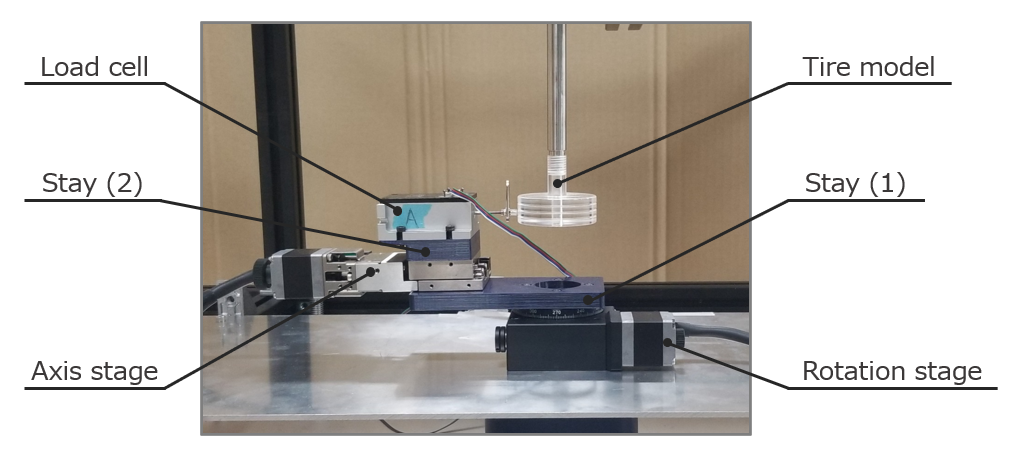
\includegraphics[width=85mm]{../images/21-2.png}
        \caption{calibration device}
    \end{center}
\end{figure}

\newpage

\section{実験方法}
作用力測定装置の性能を調べるにあたり,結果の再現性・一般性を保証するために
実験を複数回行う必要がある.ここで,大量のデータを一度にプログラムで処理できるようにするため
手順を以下のように定めた.\\

\subsection{実験手順}

\begin{enumerate}[(1)]
    \item [$\blacksquare$]  \textgt{測定条件}
    \item サンプリング周期は5[Hz]とする
    \item ロードセルをマイクロステージを用いて 0.03 [mm] ずつ移動させ,ひずみセンサ,\\
          ロードセルの出力電圧を測定する
    \item 基準を0 [mm]として,0.03 [mm],0.06 [mm],0.09 [mm],0.12 [mm]の計4回移動させる
\end{enumerate}

\begin{enumerate}[(1)]
    \item [$\blacksquare$]  \textgt{測定準備}
    \item 自動回転ステージを用いてロードセルを測定する角度に固定する
    \item 自動一軸ステージを用いてロードセルが供試体に接触する位置を0.01[mm]単位で特定する
    \item 接触する前の位置を基準に測定を開始する
\end{enumerate}

\begin{enumerate}[(1)]
    \item [$\blacksquare$]  \textgt{測定手順}
    \item 測定開始から60秒間待機する
    \item 40秒間の出力電圧の測定
    \item 60秒間の自動ステージ動作時間 (※ 自動ステージ動作後,電圧の安定を図るため)
    \item (2),(3)の作業を5回繰り返す (100秒周期) (※ 5回目はロードセル,供試体を非接触状態にする)
\end{enumerate}

\subsection{実験条件}

また,本実験では以下のTable 1のように条件を定めた.

\begin{table}[htbp]
    \scalefont{0.8}
    \begin{center}
        \caption{Experiment conditions}
        \begin{tabular}{|p{30mm}|p{20mm}|p{30}|}
            \hline
            \multicolumn{1}{|c|}{}                 & \multicolumn{1}{|c|}{\textgt{Condition number}} & \multicolumn{1}{|c|}{\textgt{Remarks}}          \\ \hline
            \multicolumn{1}{|c|}{Angle direction}  & \multicolumn{1}{|c|}{24}                        & \multicolumn{1}{|c|}{Mesurement every 15 [deg]} \\ \hline
            \multicolumn{1}{|c|}{Number of trials} & \multicolumn{1}{|c|}{5}                         & \multicolumn{1}{|c|}{}                          \\ \hline
        \end{tabular}
    \end{center}
\end{table}

\section{補正理論}

性能評価実験を行う上で,回流水槽の持つ座標系A ($x-y$),作用力測定装置の持つ座標系B ($x'-y'$),
校正実験装置の持つ座標系C ($x''-y''$)の間に以下のFig.3のような関係となる.

\begin{figure}[htbp]
    \begin{center}
        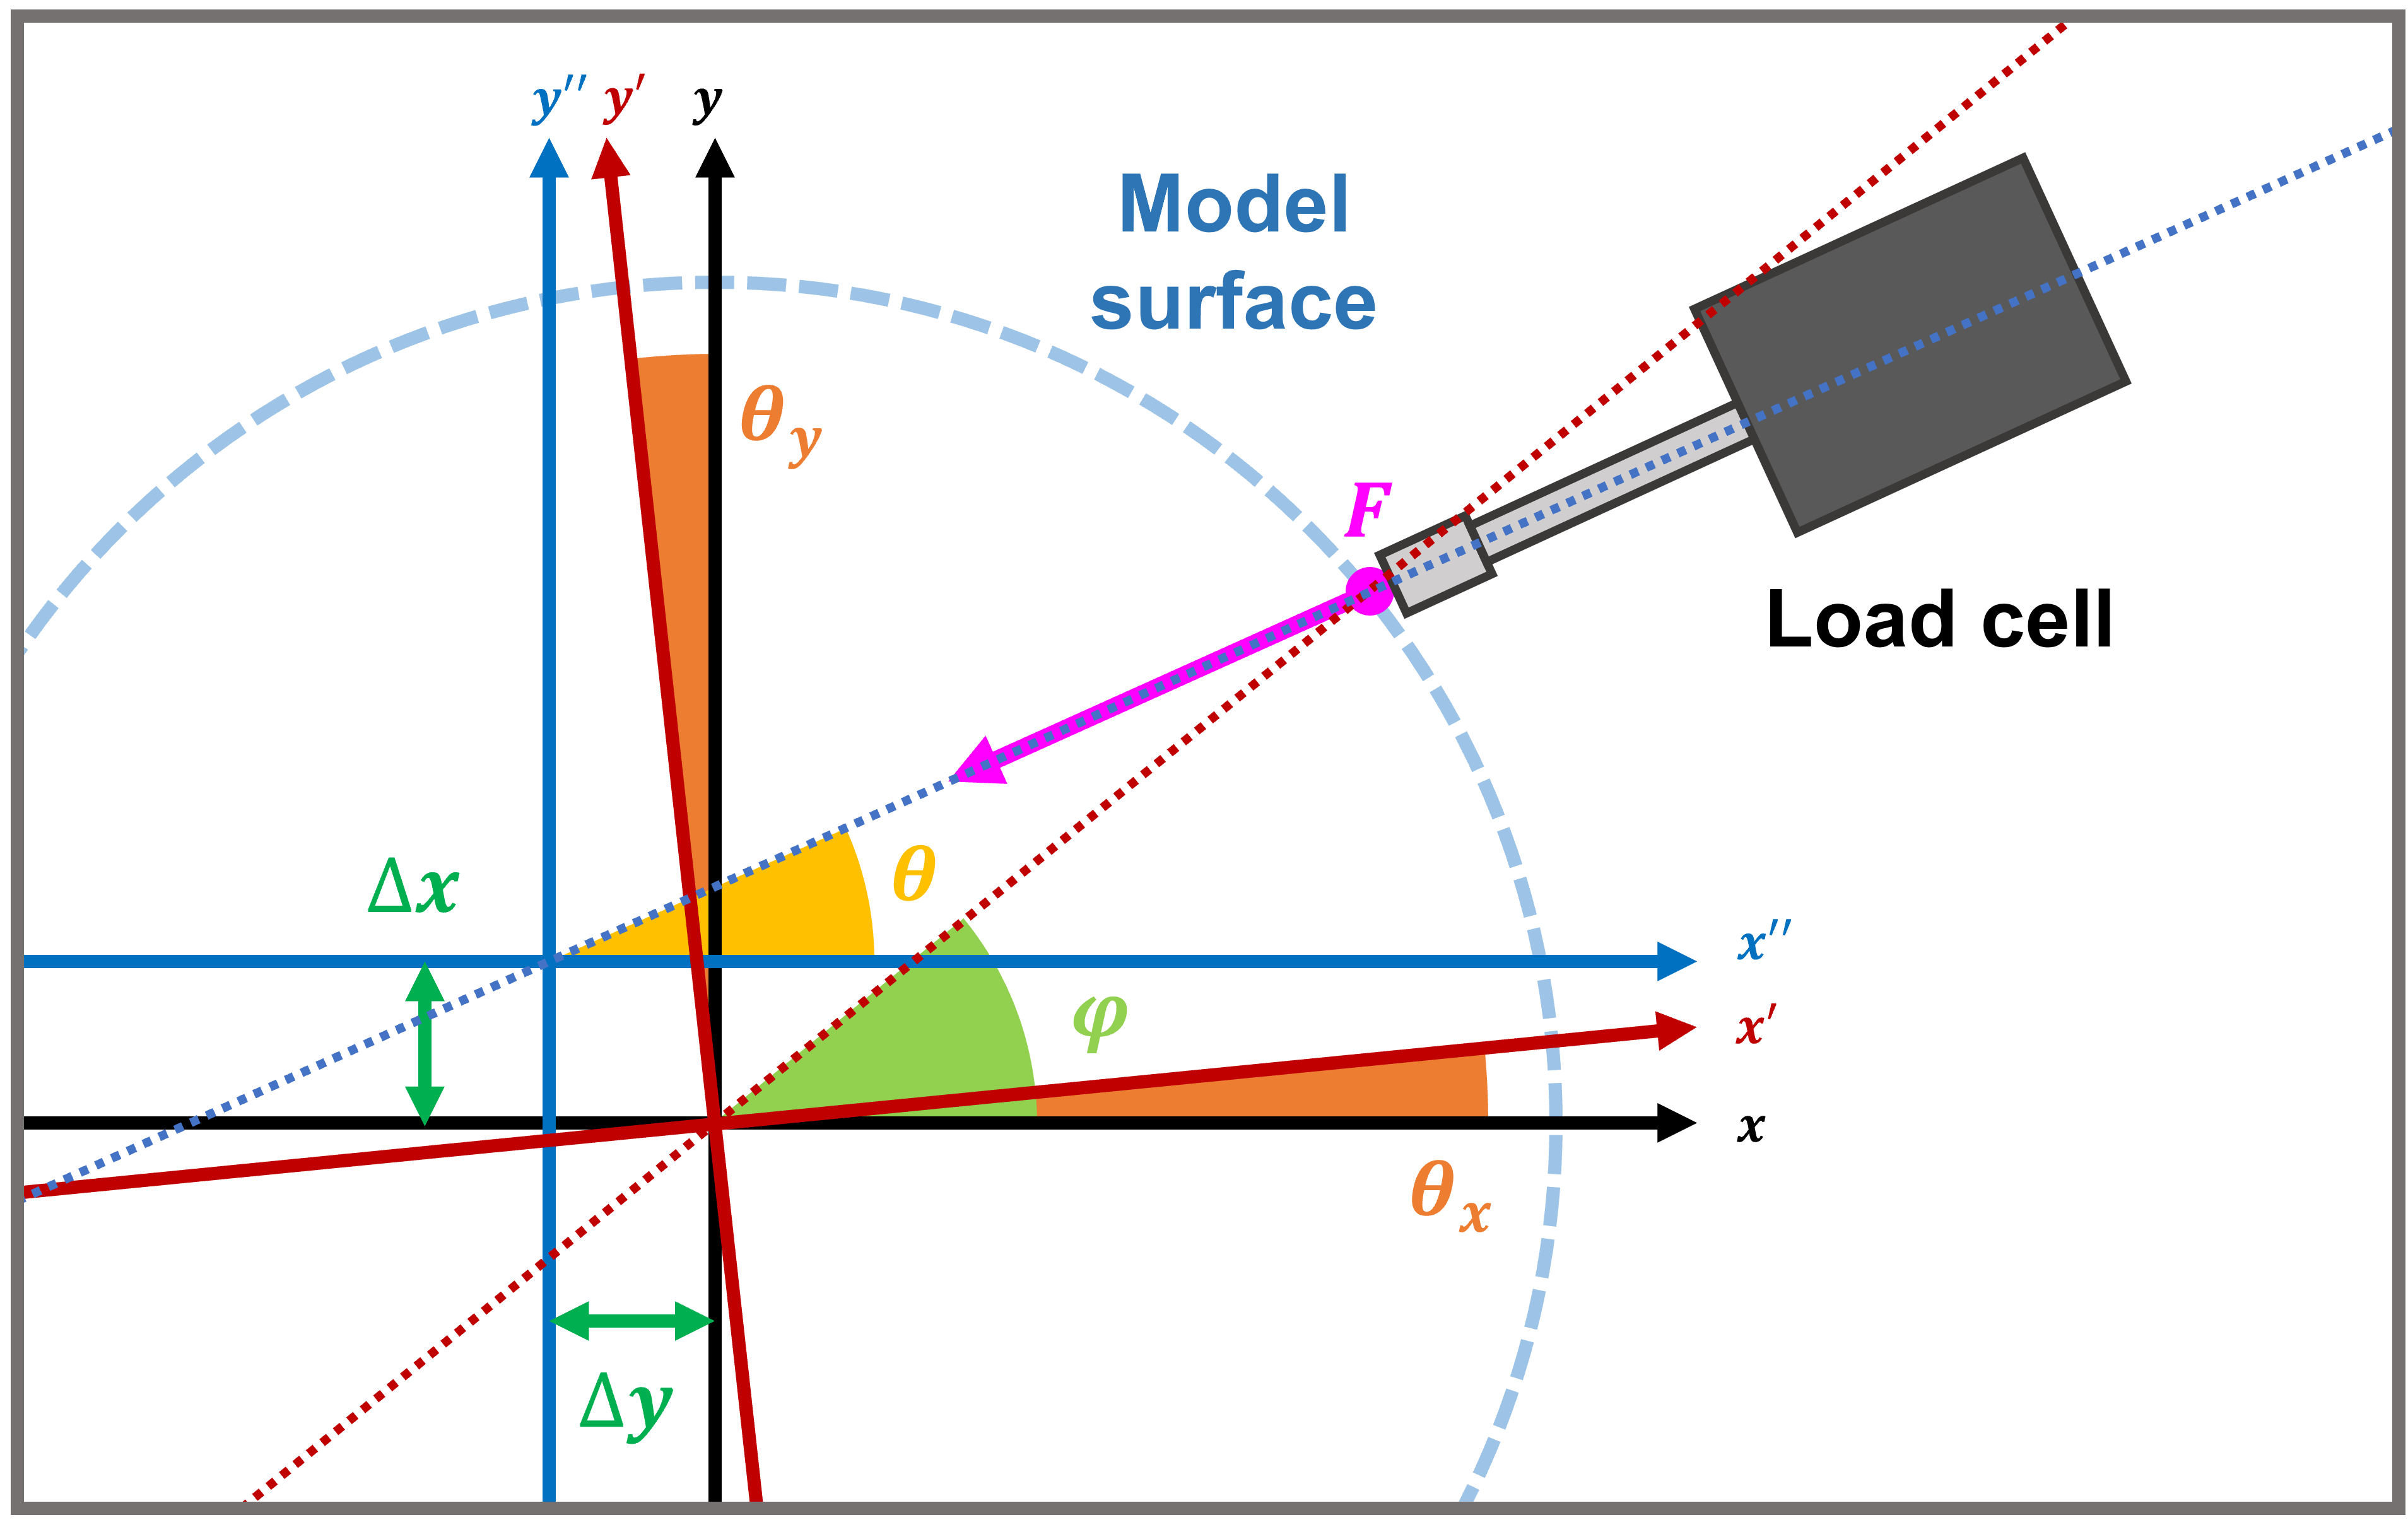
\includegraphics[width=80mm]{../images/31-1.png}
        \caption{Relationshp of coodinate system}
    \end{center}
\end{figure}

ここで,座標系Aに沿った出力電圧を得ることが目的であるが,
上記の関係性から,実験によって取得できるデータは以下ような特徴を持つ.

\begin{itemize}
    \item [$\bullet$] 回転角$\theta_x$,$\theta_y$の影響により,座標系Aに沿った出力電圧を得ることができない
    \item [$\bullet$] オフセット$\Delta x$,$\Delta y$の影響により,本来の作用力の与えられる角度は実験時のものと異なる.
\end{itemize}

したがって,作用力測定装置から得られる出力電圧を評価するためには
上記の影響を考慮し補正処理を行う必要がある.\\

\subsection{出力電圧勾配}

作用力測定装置の評価にあたり,作用力測定装置に取り付けられた2組のひずみセンサ
および校正実験の際に作用力を与えるロードセルの出力電圧の対応関係を調べることで評価を行う.
ここで,作用力測定装置において抗力方向のひずみセンサの出力電圧を$V_d$,揚力方向を$V_l$,
ロードセルの出力電圧を$V$とするとき,抗力方向の出力電圧勾配を$v_d$,
揚力方向の出力電圧勾配を$v_l$として以下のように表す.

\begin{align*}
    v_d &= V_d / V \\
    v_l &= V_l / V
\end{align*}

\newpage

\subsection{座標系の回転における補正理論}
オフセットが存在しない場合($\Delta x = 0$,$\Delta y = 0$)を考える.
このとき,座標系Bに沿った出力電圧勾配を$v_d$,$v_l$として,
回転角 $\theta_x$,$\theta_y$ が既知のとき,座標系Aにおける出力電圧勾配$v_x$,$v_y$は以下のように表される.

\begin{align*}
    v_x & = \frac{v_d \cos \theta_y - v_l \sin \theta_x}{\sin \theta_x \sin \theta_y + \cos \theta_x \cos \theta_y}                                                                                   \\
    v_y & = - \frac{1}{\tan \theta_x} \; \left(\frac{v_d \cos \theta_y - v_l \sin \theta_x}{\sin \theta_x \sin \theta_y + \cos \theta_x \cos \theta_y}\right) + \frac{|v_d|}{\sin \theta_x} \\
\end{align*}

\noindent $\blacksquare$ \textgt{テストデータへの適用 [1]}

補正理論をテストデータへと適用した.
ここで,回転角$\theta_x = 15\;\mathrm{[deg]}$,$\theta_y = 20\;\mathrm{[deg]}$としたときの
テストデータをFig.4に,その補正結果をFig.5に示す.
なお,回転角は結果に離散フーリエ変換を適用し,
波数1の成分について位相角を求めることで算出することが可能である.

\begin{figure}[htbp]
    \begin{center}
        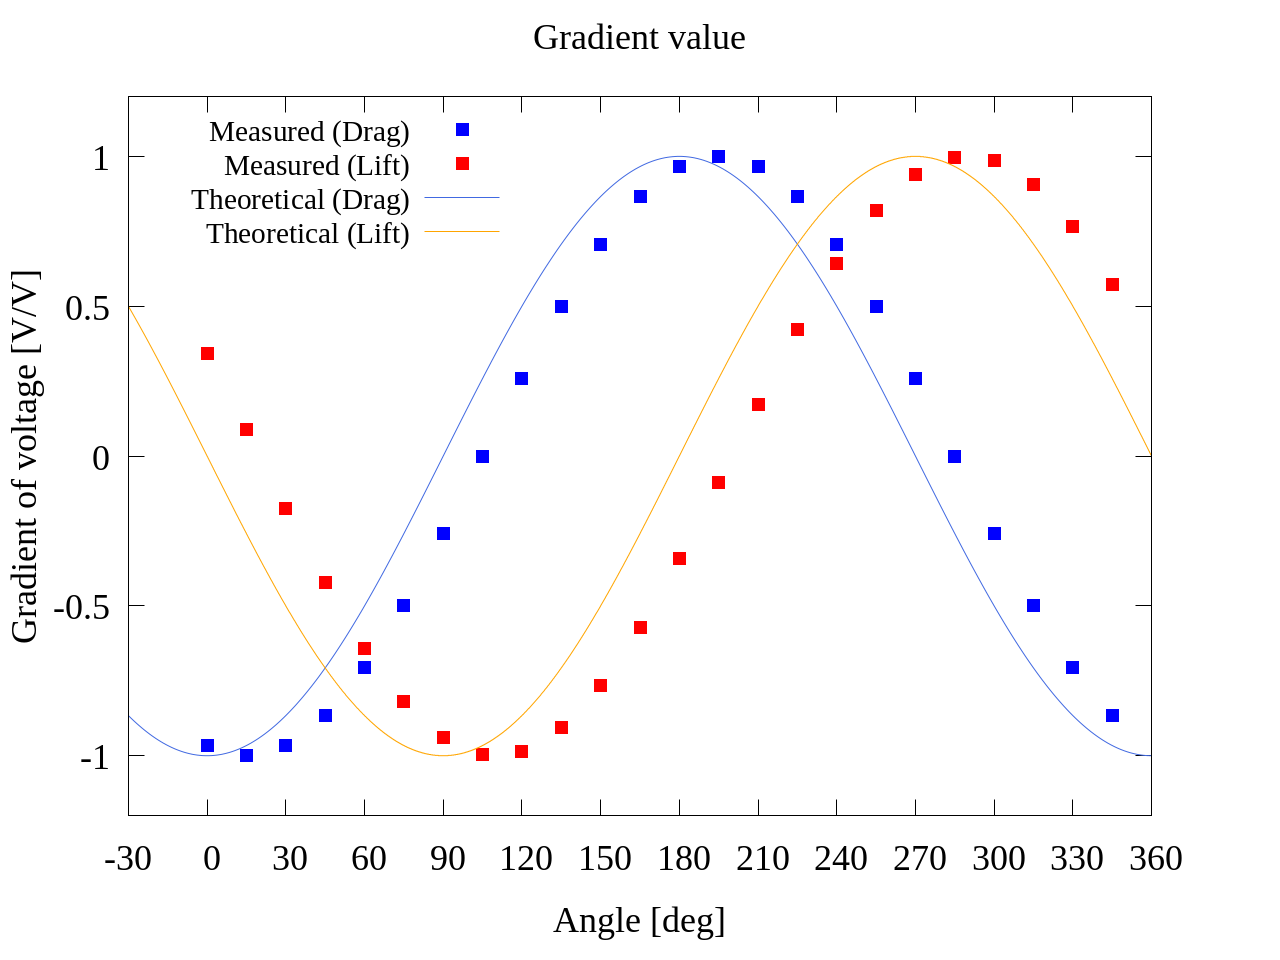
\includegraphics[width=80mm]{../../../02_workspace/result/rotation_tx=15.0_ty=20.0/plot/20/20_adjust-value.png}
        \caption{Test data [1] ($\theta_x = 15\;\mathrm{[deg]}$,$\theta_y = 20\;\mathrm{[deg]}$)}
        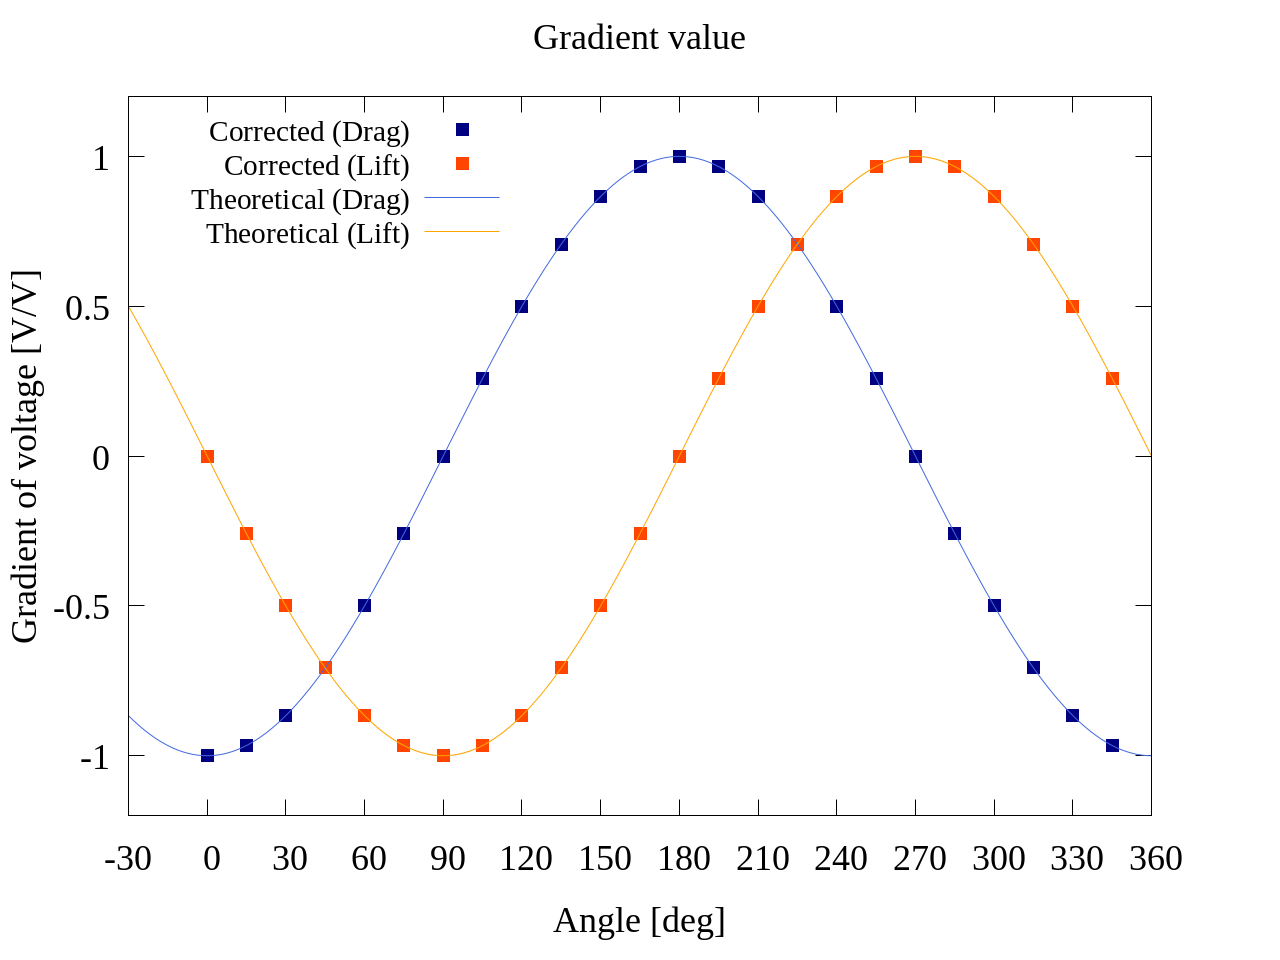
\includegraphics[width=80mm]{../../../02_workspace/result/rotation_tx=15.0_ty=20.0/plot/21/21-4_summary.png}
        \caption{Test data [1] : Rotation corrected}
    \end{center}
\end{figure}

\subsection{座標系のオフセットにおける補正理論}
回転角が存在しない場合($\theta_x=0$,$\theta_y=0$)を考える.
このとき,座標系Cに沿った出力電圧勾配を$v_d$,$v_l$として,
オフセット $\Delta x$,$\Delta y$,作用力の角度$\theta$ ,タイヤモデルの半径$r$
が既知のとき,座標系Aにおける出力電圧勾配$v_x$,$v_y$は以下のように表される.

\begin{align*}
    \alpha  & = \theta - \varphi = \sin^{-1} \left( \frac{\Delta x \sin \theta - \Delta y \cos \theta}{r} \right)       \\
    v_{x}   & = \frac{1}{\cos \alpha} v_d \\
    v_{y}   & = \frac{1}{\cos \alpha} v_l \\
\end{align*}

\noindent $\blacksquare$ \textgt{テストデータへの適用 [2]}

補正理論をテストデータへと適用した.
ここで,オフセット$\Delta x = 10\;\mathrm{[mm]}$,$\Delta y = 5\;\mathrm{[mm]}$としたときの
テストデータをFig.6に,その補正結果をFig.7に示す.
なお,オフセットは実験時に測定することで求めることができる.

\begin{figure}[htbp]
    \begin{center}
        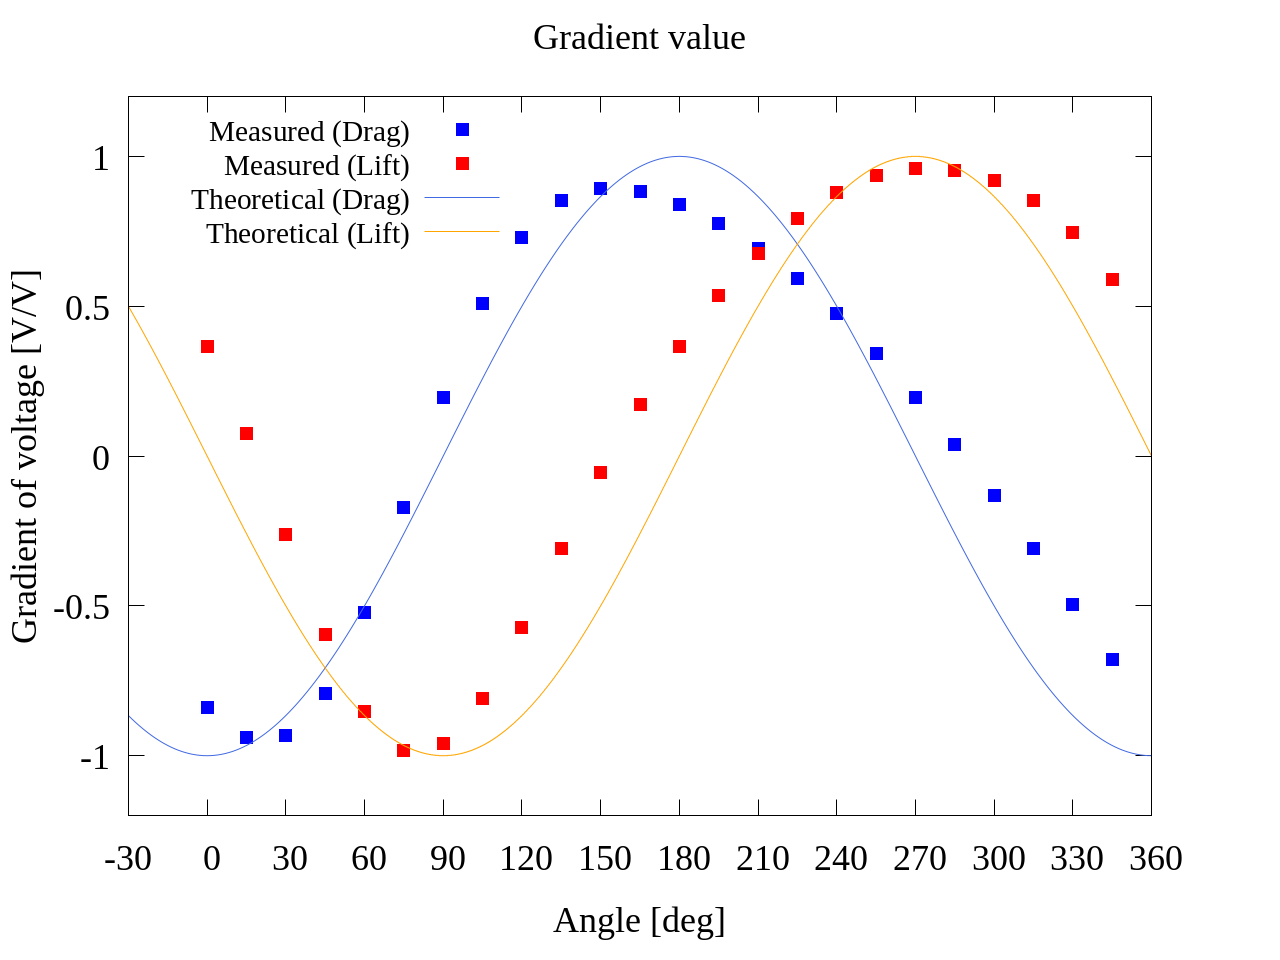
\includegraphics[width=80mm]{../../../02_workspace/result/offset_dx=10.0_dy=5.0/plot/20/20_adjust-value.png}
        \caption{Test data [2] ($\Delta x = 10\;\mathrm{[mm]}$,$\Delta y = 5\;\mathrm{[mm]}$)}
        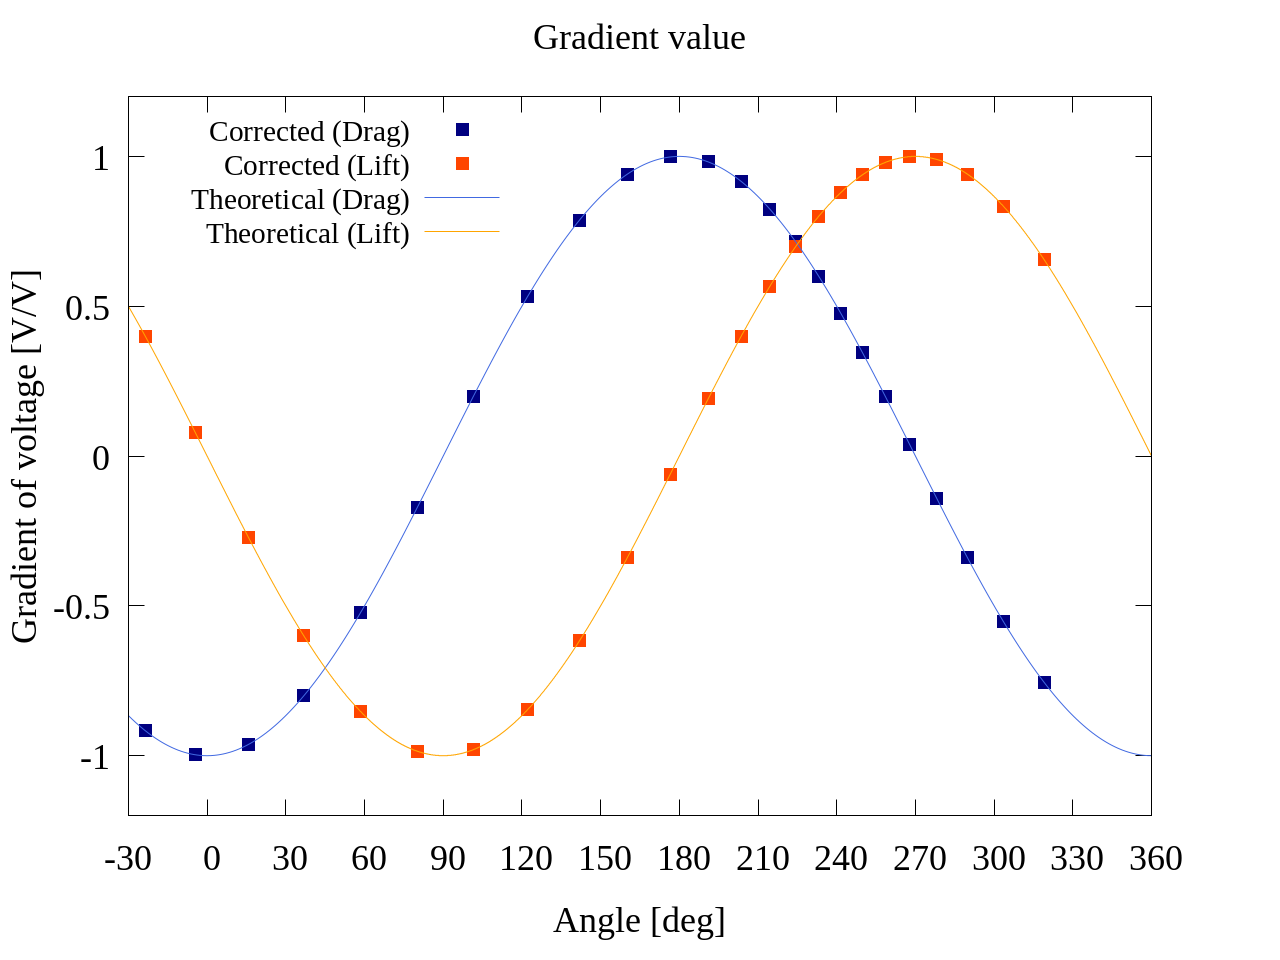
\includegraphics[width=80mm]{../../../02_workspace/result/offset_dx=10.0_dy=5.0/plot/21/21-2_summary_offset.png}
        \caption{Test data [2] : Offset corrected}
    \end{center}
\end{figure}


\subsection{複合状態における補正理論}

実際の回転角$\theta_x$,$\theta_y$およびオフセット$\Delta x$,$\Delta y$が存在する場合について考える.
ここで,Fig.7をみるとオフセット補正後の結果は不等間隔になることがわかる.
これは作用力を与えるとき,みかけの角度$\theta$と実際の角度$\varphi$が異なるためである.
このとき,回転角を求める際に離散フーリエ変換を用いて回転角を特定し,補正理論を適用するが
データが不等間隔であるため離散フーリエ変換を適用できない.
したがって,等間隔のデータを得るためにラグランジュ補間公式を用いて等間隔のデータを得ることとする.
一般にラグランジュ補間公式とは,$(x_1,f\left(x_1\right))$,$(x_2,f\left(x_2\right))$,
$(x_3,f \left(x_3\right))$,$\cdots$の点を通る関数$P\left(x\right)$を以下のように表す.

\begin{align*}
    P\left(x\right)    & = \sum^{n+1}_{i=1} y_i \frac{f_i\left(x\right)}{f_i \left(x_i\right)} \\
    f_i \left(x\right) & = \prod_{k \neq i} \left(x - x_k\right)\\
\end{align*}

テストデータ[2]にラグランジュ補間公式を用いて等間隔データへと補正した結果を以下のFig.9に示す.

\begin{figure}[htbp]
    \begin{center}
        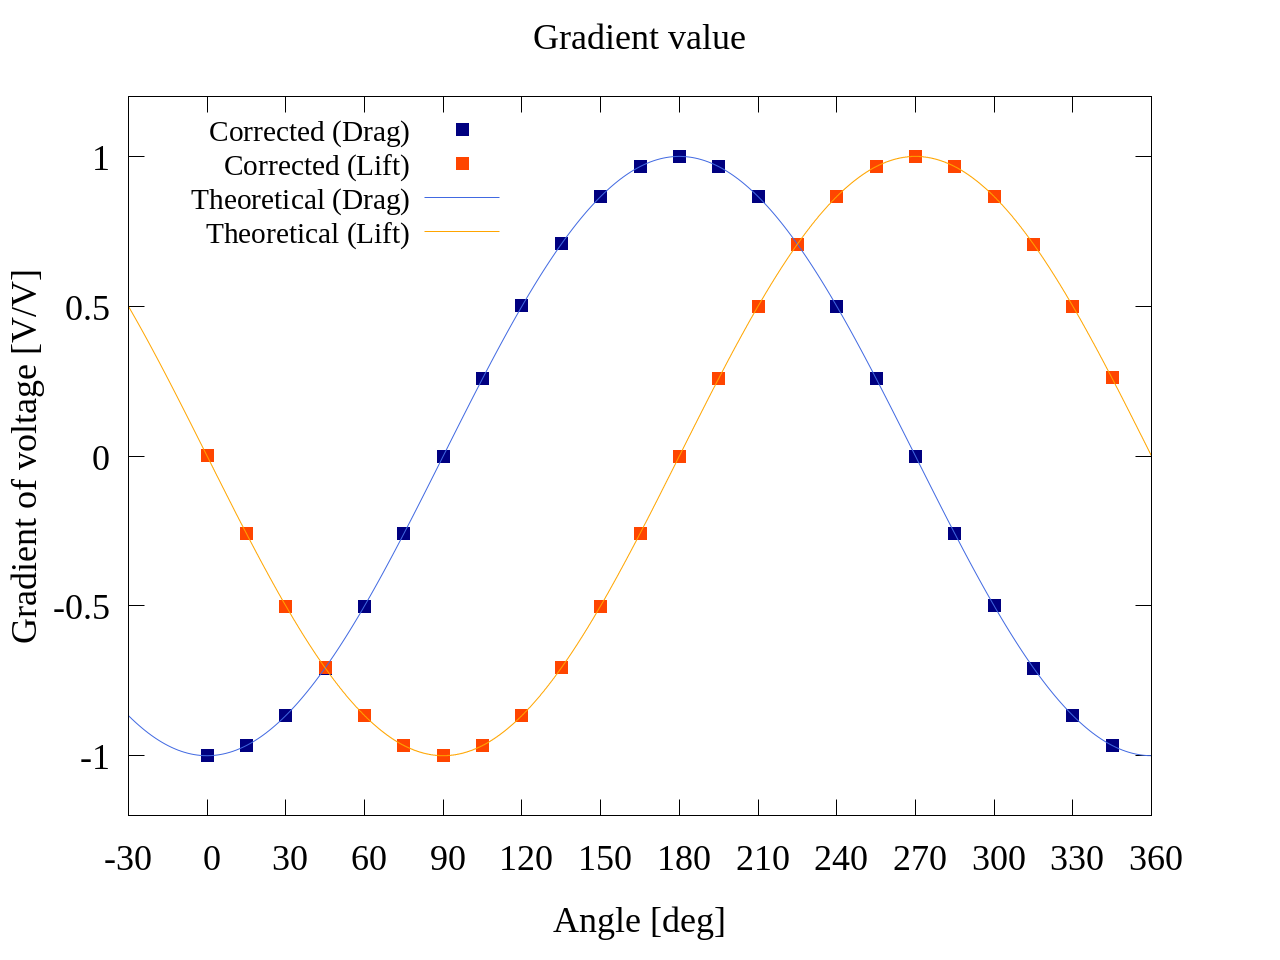
\includegraphics[width=80mm]{../../../02_workspace/result/offset_dx=10.0_dy=5.0/plot/21/21-3_summary_interpolated.png}
        \caption{Test data [2] : Lagrange interpolated}
    \end{center}
\end{figure}

\newpage

\noindent $\blacksquare$ \textgt{テストデータへの適用 [3]}

補正理論についてテストデータを作成し,その有効性を確かめる.
以下のTable 2に示すパラメータを用いてテストデータを作成した.

\begin{table}[htbp]
    \begin{center}
        \caption{Test data conditions [3]}
        \begin{tabular}{|p{20mm}|p{20mm}|p{20mm}|p{20mm}|}
            \hline
            \multicolumn{1}{|c|}{$\theta_x$ [deg]} & \multicolumn{1}{|c|}{$\theta_y$ [deg]} & \multicolumn{1}{|c|}{$\Delta x$ [mm]} & \multicolumn{1}{|c|}{$\Delta y$ [mm]} \\ \hline
            \multicolumn{1}{|c|}{10.0}                              & \multicolumn{1}{|c|}{-5.0}                              & \multicolumn{1}{|c|}{5.00}                          & \multicolumn{1}{|c|}{-2.50}                         \\ \hline
        \end{tabular}
    \end{center}
\end{table}

作成したテストデータを以下のFig.9に示す.

\begin{figure}[htbp]
    \begin{center}
        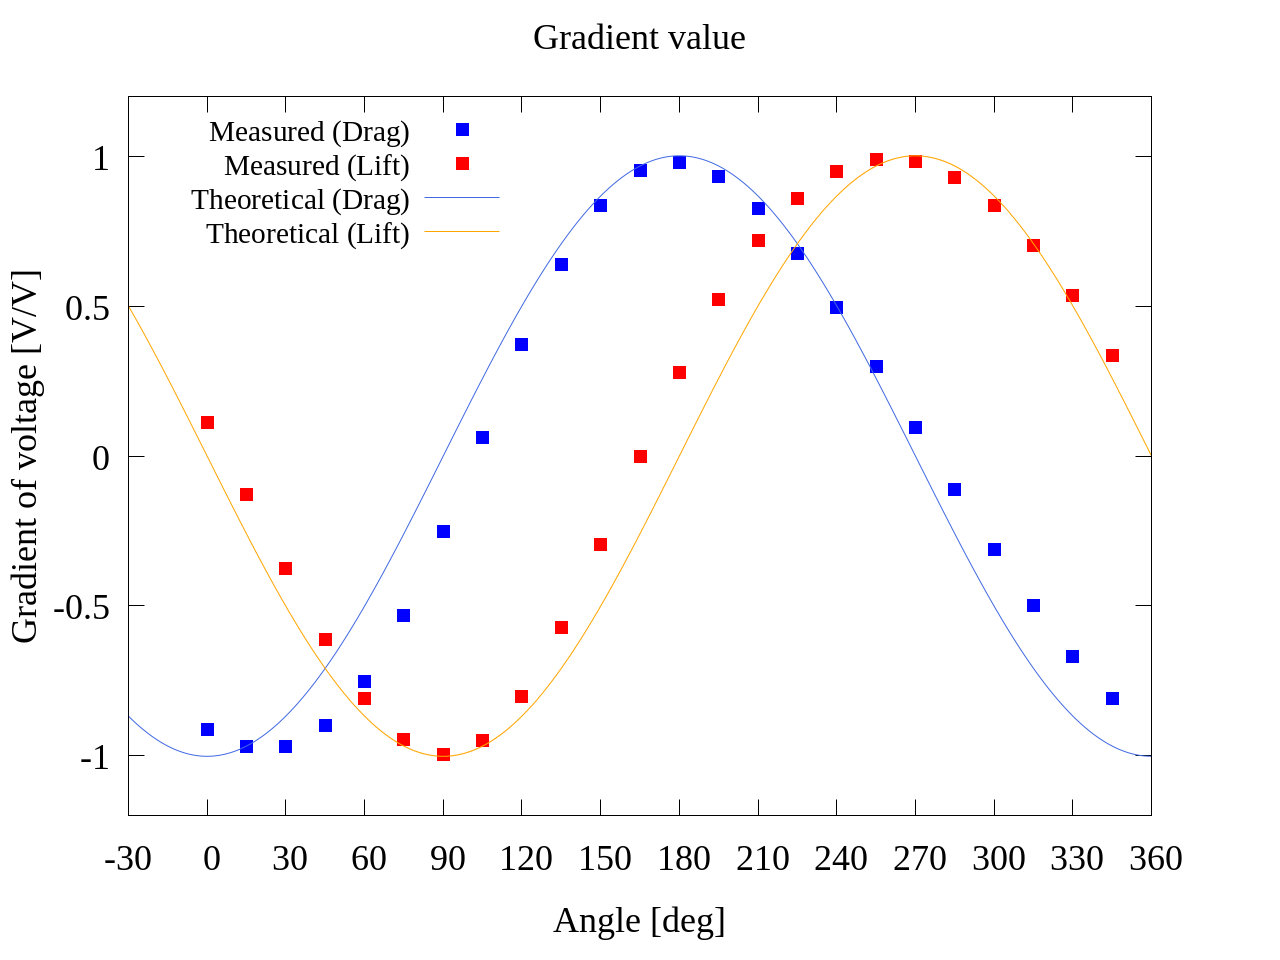
\includegraphics[width=80mm]{../../../02_workspace/result/simulation_tx=10.0_ty=-5.0_dx=5.00_dy=-2.50/plot/20/20_adjust-value.png}
        \caption{Test data [3]}
    \end{center}
\end{figure}

\noindent $\blacksquare$ \textgt{オフセット補正の適用}

テストデータ[3]にオフセット補正を適用した結果を以下のFig.10に示す.

\begin{figure}[htbp]
    \begin{center}
        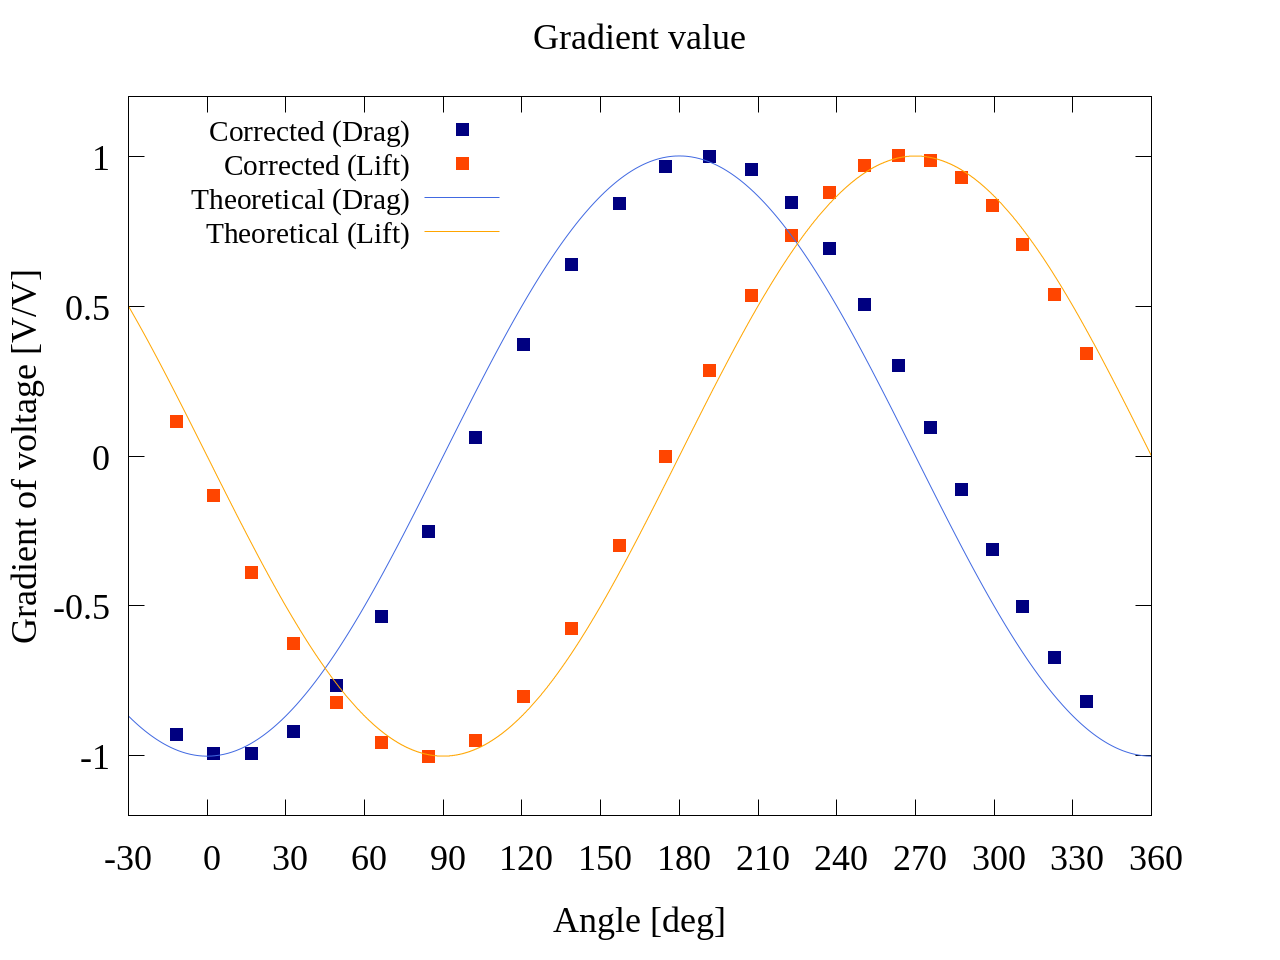
\includegraphics[width=80mm]{../../../02_workspace/result/simulation_tx=10.0_ty=-5.0_dx=5.00_dy=-2.50/plot/21/21-2_summary_offset.png}
        \caption{Test data [3] : Offset corrected}
    \end{center}
\end{figure}

\newpage

\noindent $\blacksquare$ \textgt{ラグランジュ補間公式の適用}

テストデータ[3]にラグランジュ補間公式を適用した結果を以下のFig.11に示す.

\begin{figure}[htbp]
    \begin{center}
        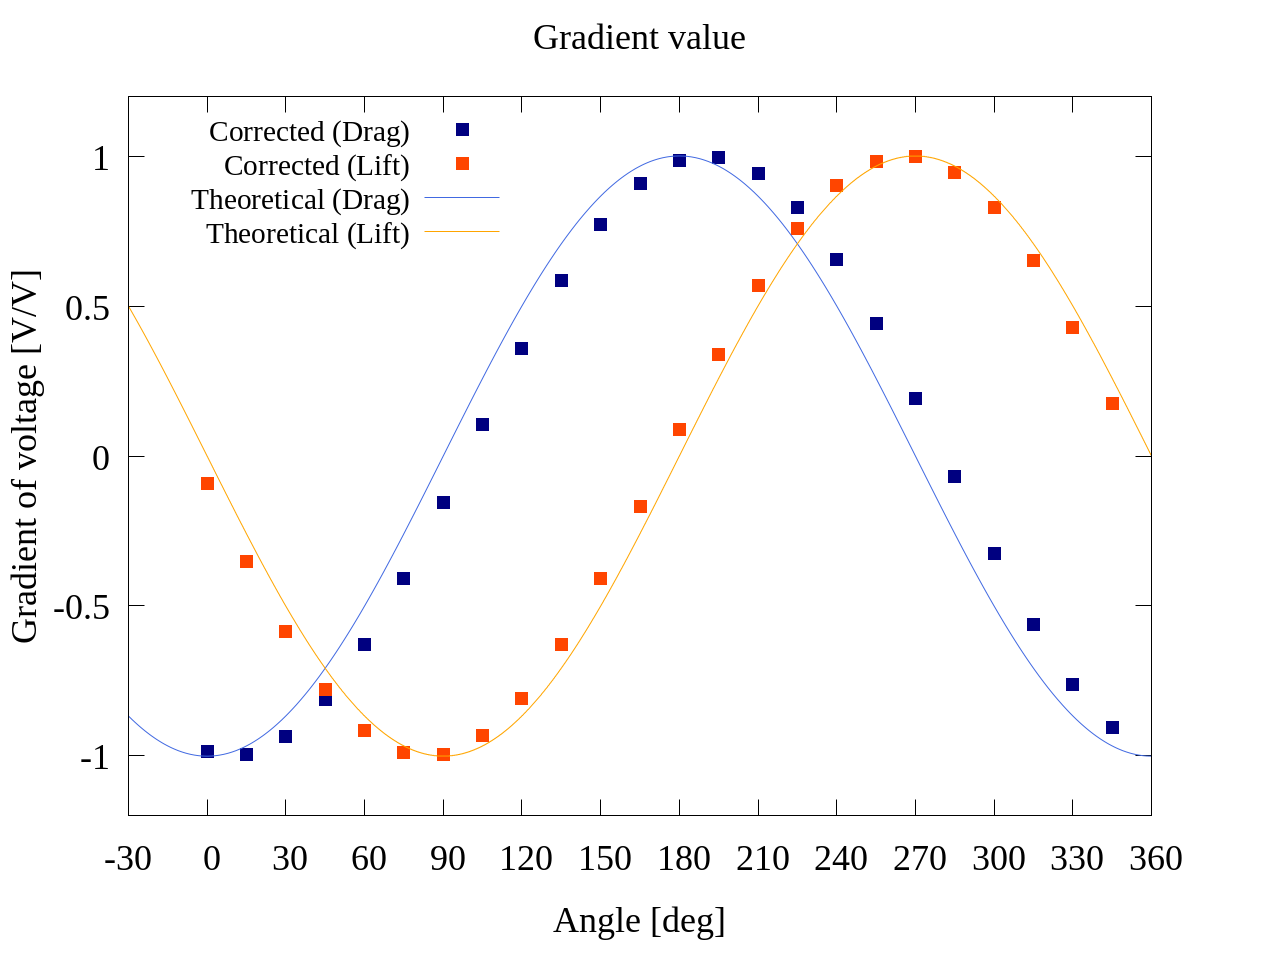
\includegraphics[width=80mm]{../../../02_workspace/result/simulation_tx=10.0_ty=-5.0_dx=5.00_dy=-2.50/plot/21/21-3_summary_interpolated.png}
        \caption{Test data [3] : lagrange corrected}
    \end{center}
\end{figure}

\noindent $\blacksquare$ \textgt{回転補正の適用}

テストデータ[3]に回転補正を適用した結果を以下のFig.12に示す.

\begin{figure}[htbp]
    \begin{center}
        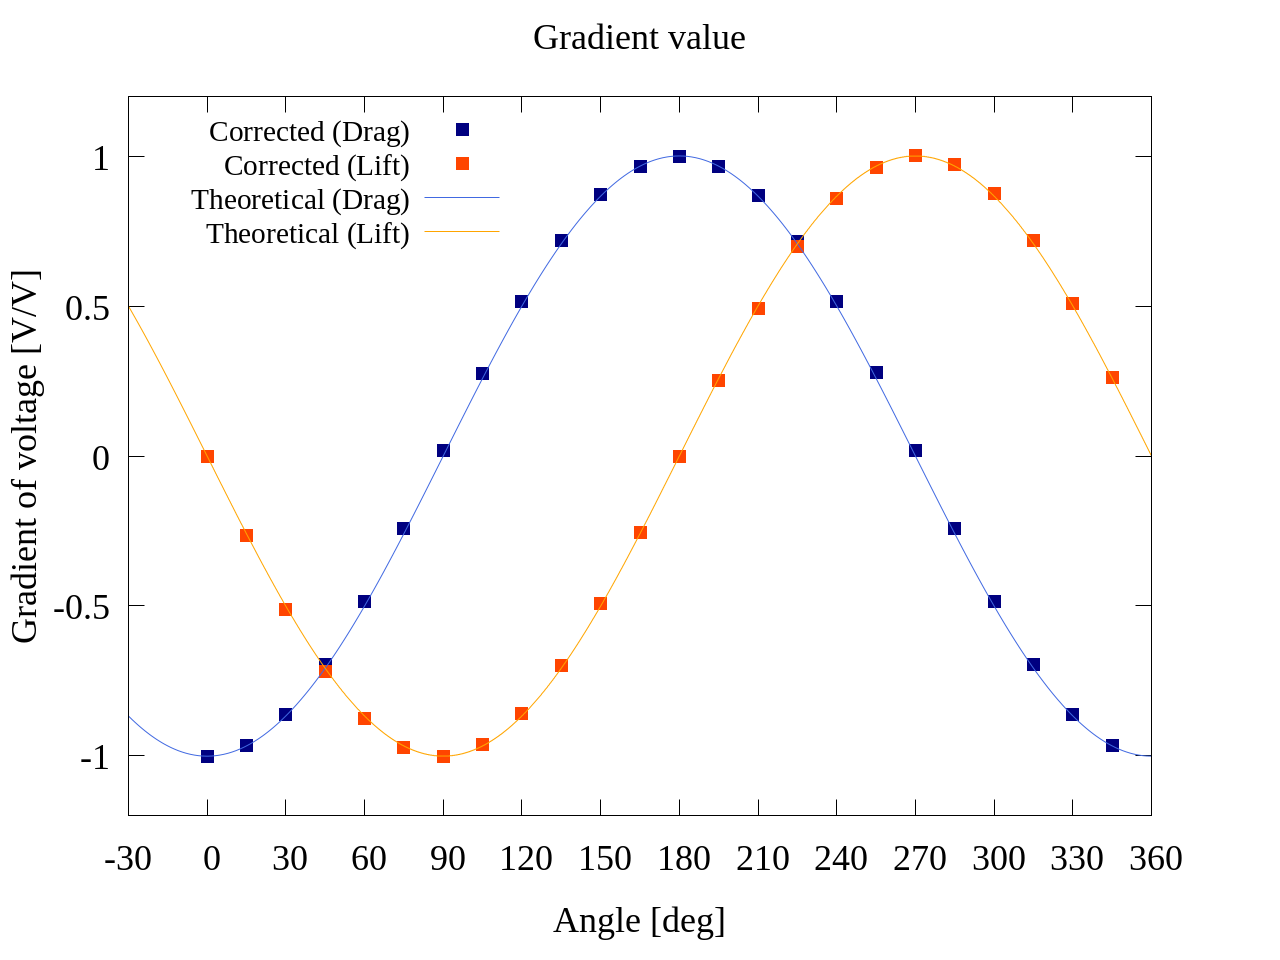
\includegraphics[width=80mm]{../../../02_workspace/result/simulation_tx=10.0_ty=-5.0_dx=5.00_dy=-2.50/plot/21/21-4_summary.png}
        \caption{Test data [3] : Rotation corrected}
    \end{center}
\end{figure}

また,このとき算出された回転角$\theta_x$,$\theta_y$を以下のTable 3に示す.

\begin{table}[htbp]
    \begin{center}
        \caption{Specified rotation angle [Case 7]}
        \begin{tabular}{|p{20mm}|p{20mm}|}
            \hline
            \multicolumn{1}{|c|}{$\theta_x$ [deg]} & \multicolumn{1}{|c|}{$\theta_y$ [deg]} \\ \hline
            \multicolumn{1}{|c|}{7.757}           & \multicolumn{1}{|c|}{5.019}           \\ \hline
        \end{tabular}
    \end{center}
\end{table}

ここで,テストデータ[3]の作成に使用したパラメータと一致しないのは,
ラグランジュ補間公式の適用の際に発生する誤差の影響と考えられる.

\section{実験結果と考察}

実施した実験結果を以下のTable 4,Fig.13に示す.
なお,この結果は5回の平均値を示している.

\begin{table}[htbp]
    \begin{center}
        \scalefont{0.95}
        \caption{Average of experimental data (table)}
        \begin{tabular}{|p{20mm}|p{20mm}|p{20mm}|}
            \hline
            \multicolumn{1}{|c|}{\textgt{varphi [deg]}} & \multicolumn{1}{|c|}{\textgt{$v_d$ [V/V]}} & \multicolumn{1}{|c|}{\textgt{$v_l$ [V/V]}} \\ \hline
            \multicolumn{1}{|c|}{0}                    & \multicolumn{1}{|r|}{-0.627}               & \multicolumn{1}{|r|}{ 0.063}               \\ \hline
            \multicolumn{1}{|c|}{15}                   & \multicolumn{1}{|r|}{-0.617}               & \multicolumn{1}{|r|}{-0.103}               \\ \hline
            \multicolumn{1}{|c|}{30}                   & \multicolumn{1}{|r|}{-0.566}               & \multicolumn{1}{|r|}{-0.261}               \\ \hline
            \multicolumn{1}{|c|}{45}                   & \multicolumn{1}{|r|}{-0.479}               & \multicolumn{1}{|r|}{-0.405}               \\ \hline
            \multicolumn{1}{|c|}{60}                   & \multicolumn{1}{|r|}{-0.365}               & \multicolumn{1}{|r|}{-0.508}               \\ \hline
            \multicolumn{1}{|c|}{75}                   & \multicolumn{1}{|r|}{-0.226}               & \multicolumn{1}{|r|}{-0.582}               \\ \hline
            \multicolumn{1}{|c|}{90}                   & \multicolumn{1}{|r|}{-0.038}               & \multicolumn{1}{|r|}{-0.624}               \\ \hline
            \multicolumn{1}{|c|}{105}                  & \multicolumn{1}{|r|}{0.131}                & \multicolumn{1}{|r|}{-0.618}               \\ \hline
            \multicolumn{1}{|c|}{120}                  & \multicolumn{1}{|r|}{0.296}                & \multicolumn{1}{|r|}{-0.560}               \\ \hline
            \multicolumn{1}{|c|}{135}                  & \multicolumn{1}{|r|}{0.425}                & \multicolumn{1}{|r|}{-0.474}               \\ \hline
            \multicolumn{1}{|c|}{150}                  & \multicolumn{1}{|r|}{0.536}                & \multicolumn{1}{|r|}{-0.345}               \\ \hline
            \multicolumn{1}{|c|}{165}                  & \multicolumn{1}{|r|}{0.611}                & \multicolumn{1}{|r|}{-0.189}               \\ \hline
            \multicolumn{1}{|c|}{180}                  & \multicolumn{1}{|r|}{0.643}                & \multicolumn{1}{|r|}{-0.011}               \\ \hline
            \multicolumn{1}{|c|}{195}                  & \multicolumn{1}{|r|}{0.620}                & \multicolumn{1}{|r|}{0.156}                \\ \hline
            \multicolumn{1}{|c|}{210}                  & \multicolumn{1}{|r|}{0.561}                & \multicolumn{1}{|r|}{0.294}                \\ \hline
            \multicolumn{1}{|c|}{225}                  & \multicolumn{1}{|r|}{0.487}                & \multicolumn{1}{|r|}{0.402}                \\ \hline
            \multicolumn{1}{|c|}{240}                  & \multicolumn{1}{|r|}{0.399}                & \multicolumn{1}{|r|}{0.489}                \\ \hline
            \multicolumn{1}{|c|}{255}                  & \multicolumn{1}{|r|}{0.289}                & \multicolumn{1}{|r|}{0.565}                \\ \hline
            \multicolumn{1}{|c|}{270}                  & \multicolumn{1}{|r|}{0.163}                & \multicolumn{1}{|r|}{0.616}                \\ \hline
            \multicolumn{1}{|c|}{285}                  & \multicolumn{1}{|r|}{0.006}                & \multicolumn{1}{|r|}{0.641}                \\ \hline
            \multicolumn{1}{|c|}{300}                  & \multicolumn{1}{|r|}{-0.181}               & \multicolumn{1}{|r|}{0.615}                \\ \hline
            \multicolumn{1}{|c|}{315}                  & \multicolumn{1}{|r|}{-0.353}               & \multicolumn{1}{|r|}{0.532}                \\ \hline
            \multicolumn{1}{|c|}{330}                  & \multicolumn{1}{|r|}{-0.490}               & \multicolumn{1}{|r|}{0.406}                \\ \hline
            \multicolumn{1}{|c|}{345}                  & \multicolumn{1}{|r|}{-0.582}               & \multicolumn{1}{|r|}{0.237}                \\ \hline
        \end{tabular}
    \end{center}
\end{table}

\begin{figure}[htbp]
    \begin{center}
        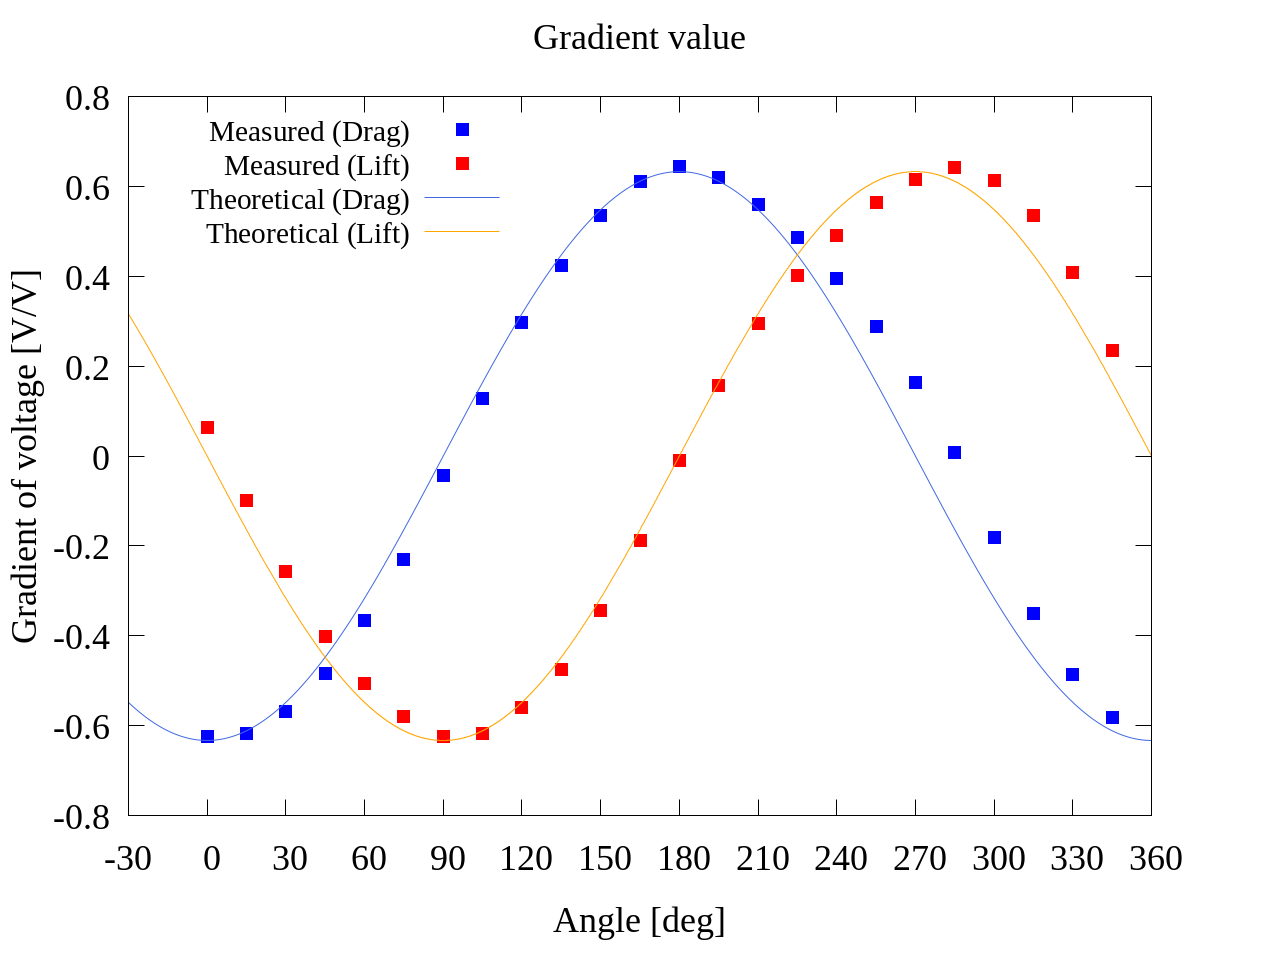
\includegraphics[width=80mm]{../../../02_workspace/result/2-ex/plot/20/20_adjust-value.png}
        \caption{Average of experimental data (graph)}
    \end{center}
\end{figure}

\newpage

また,実験時に測定したオフセット値を以下のTable 5に示す.

\begin{table}[htbp]
    \begin{center}
        \caption{Offset velue}
        \begin{tabular}{|p{30mm}|p{20mm}|p{20mm}|}
            \hline
            \multicolumn{1}{|c|}{$\Delta x$ [mm]} & \multicolumn{1}{|c|}{$\Delta y$ [mm]} \\ \hline
            \multicolumn{1}{|c|}{0.09}           & \multicolumn{1}{|c|}{0.06}           \\ \hline
        \end{tabular}
    \end{center}
\end{table}

ここで,

\section{結論}

\section{今月の進捗と2月の予定}

\end{document}